%\renewcommand{\thefootnote}{\arabic{footnote}}
\chapter{TINJAUAN PUSTAKA}
\label{BAB2:tinjauan}

Manfaatkan penggunaan perintah \verb|\label{}| untuk menjadikan suatu bab atau subbab sebagai acuan. Untuk mengacu ke bab atau subbab itu maka gunakan perintah \verb|\ref{}|. Sebagai contoh, Bab \verb|\ref{BAB1:pendahuluan}| akan mengahsilkan: Bab \ref{BAB1:pendahuluan}. Teknik yang sama juga bisa digunakan untuk mengacu ke suatu gambar atau tabel. Sebagai contoh, Gambar~\ref{fig:arsitektur} menunjukkan arsitektur dari blok \textit{Residual Networks} (ResNet).
\begin{figure}[h]
    \centering
    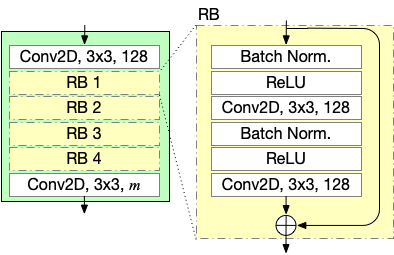
\includegraphics[scale=0.5]{BAB-2/resnet receiver.png}
    \caption{Arsitektur Blok ResNet}
    \label{fig:arsitektur}
\end{figure}

Salah cara untuk membuat tabel, seperti yang ditunjukkan pada Tabel~\ref{tab:test}, adalah dengan menggunakan \verb|longtblr| \citep{tabularray}.
\begin{longtblr}[
  caption = {Tabel yang panjang},
  label = {tab:test},
]{
  colspec = {|XX[4]|},
  rowhead = 1,
  hlines,
  row{even} = {gray9},
  row{1} = {olive9},
} 
No. & Kolom 1 \\
1  & blablabla \\
2  & blablabla \\
3  & blablabla \\
4  & blablabla \\
5  & blablabla \\
6  & blablabla \\
7  & blablabla \\
8  & blablabla \\
9  & blablabla \\
10  & blablabla \\
11  & blablabla \\
12  & blablabla \\
13  & blablabla \\
14  & blablabla \\
15  & blablabla \\
16  & blablabla \\
17  & blablabla \\
18  & blablabla \\
19  & blablabla \\
20  & blablabla \\
21  & blablabla \\
22  & blablabla \\
\end{longtblr}